\subsection{Mods}

Embora o sistema de redstone presente na versão vanilla do jogo já permita a construção de circuitos digitais relativamente complexos, algumas limitações práticas, como atraso de propagação, dificuldade de depuração e alta complexidade estrutural, motivam o uso de modificações (mods) que expandem essas capacidades.

Esses mods introduzem ferramentas e abstrações que aproximam o ambiente do jogo de um contexto mais controlado e analisável, semelhante ao de sistemas digitais reais ou simuladores de hardware. Foi utilizado o Fabric 0.19.1-1.18.2

\subsubsection{Carpet}

O mod Carpet fornece ferramentas avançadas de análise e instrumentação do jogo. Entre suas funcionalidades, destacam-se a medição de desempenho, inspeção de ticks e controle fino do comportamento do sistema.

Essas capacidades permitem observar com maior precisão a execução de circuitos de redstone, facilitando a identificação de gargalos, condições de corrida e inconsistências temporais.

\subsubsection{Wired Redstone}

O mod Wired Redstone introduz um sistema de fiação estruturado que substitui a redstone tradicional por conexões mais organizadas e previsíveis.

Diferentemente da redstone vanilla, esses fios não sofrem degradação de sinal ao longo da distância, eliminando a necessidade de repetidores.

\textbf{Principais itens:}
\begin{itemize}
    \item \textbf{Red Alloy Wire}: fio condutor básico sem perda de sinal.
    \item \textbf{Insulated Wire}: fios isolados por cor, permitindo múltiplos sinais independentes em paralelo.
    \item \textbf{Bundled Cable}: permite transmitir vários sinais simultaneamente em um único bloco (barramento multi-bit).
    \item \textbf{Gate Components}: componentes lógicos (AND, OR, NOT, etc.) integrados ao sistema de fios.
	\item \textbf{Repetidor de Redstone}: o mod adiciona uma alternativa do repetidor de redstone \textit{vanilla} com personalização do atraso em ticks gerado.
\end{itemize}

\begin{figure}[H]
   	\centering
   	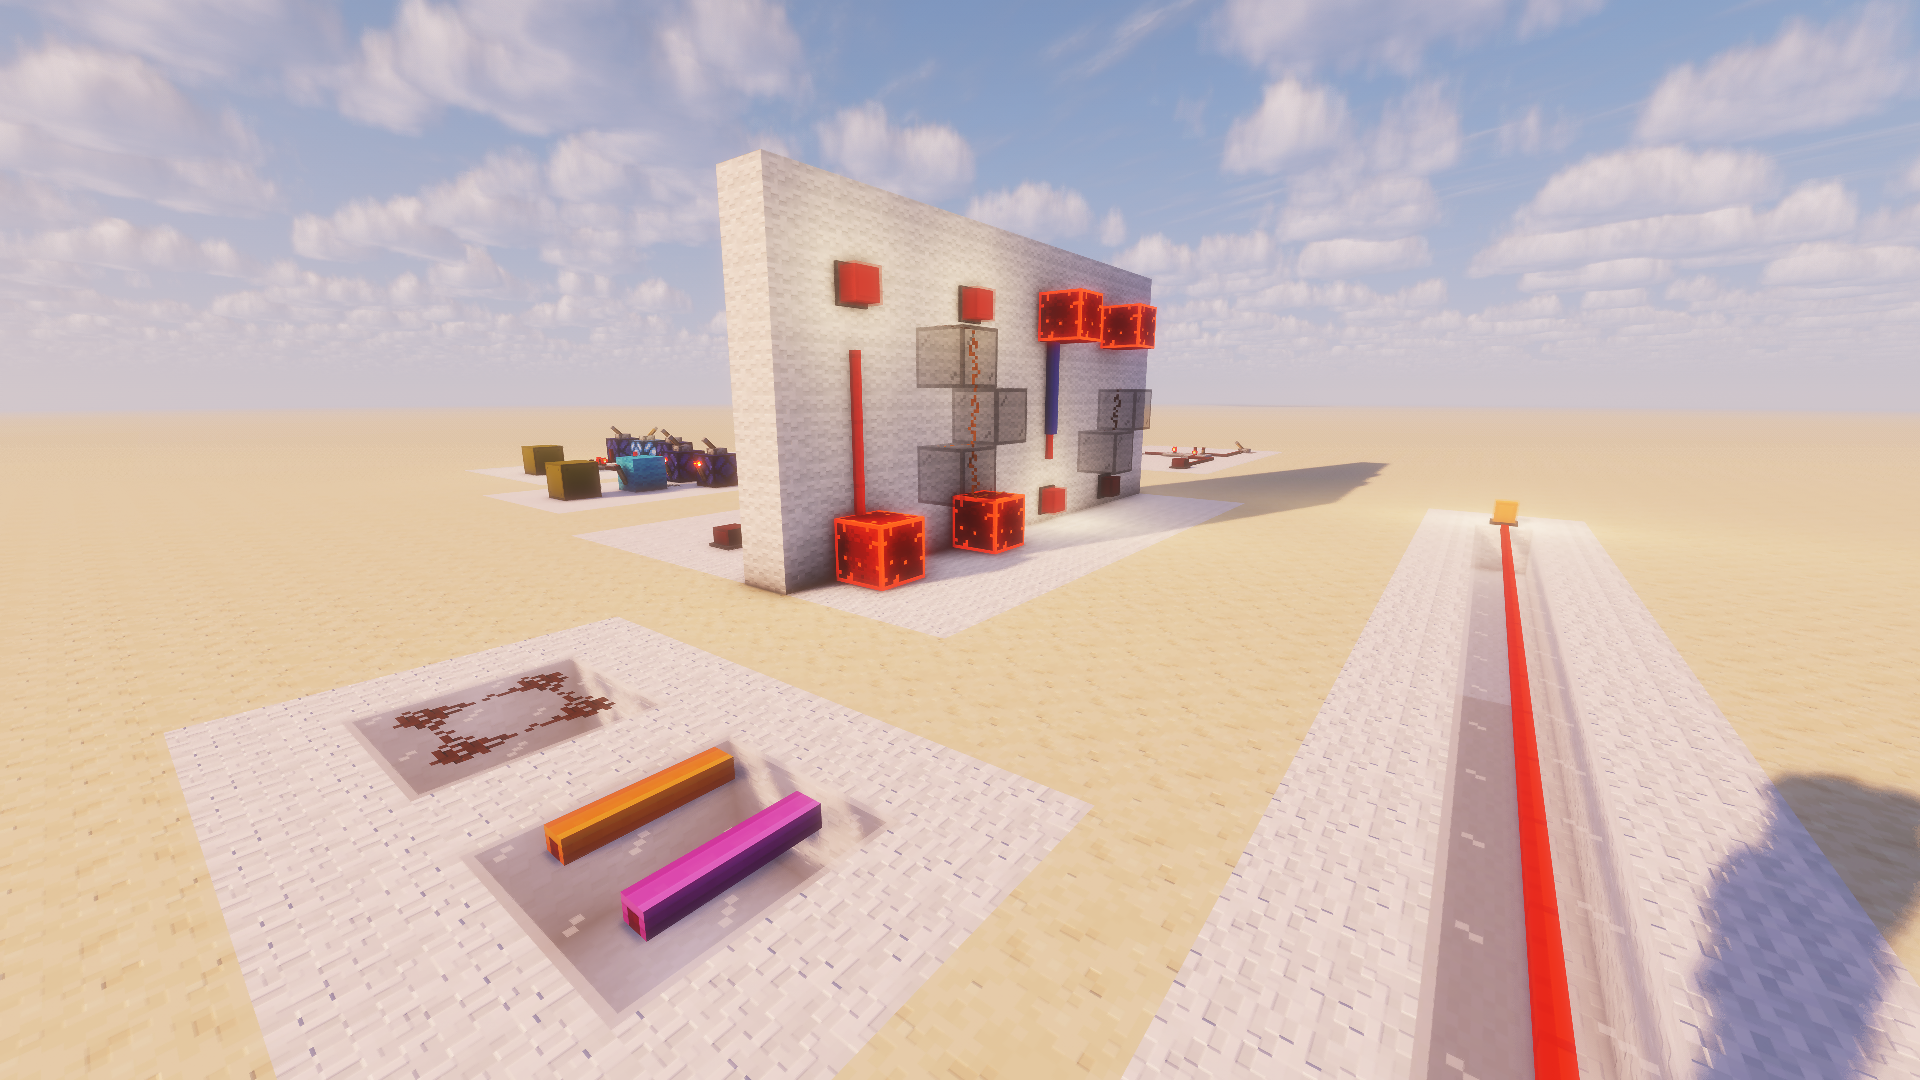
\includegraphics[width=0.7\linewidth]{images/wired-redstone.png}
  	 \caption{Fios de Redstone}
   	\label{fig:wired-redstone}
	%{\footnotesize Fonte: \url{https://autoctrls.com/datasheet-transistor/}}
\end{figure}


\subsubsection{Wireless Redstone}

O mod Wireless Redstone introduz comunicação sem fio entre componentes, eliminando completamente a necessidade de conexões físicas.

O funcionamento segue o modelo de transceptores: um transmissor envia um sinal em uma determinada frequência/canal, e receptores configurados na mesma frequência reproduzem esse sinal.

\textbf{Principais itens:}
\begin{itemize}
    \item \textbf{Transmitter}: envia sinais de redstone para um canal específico.
    \item \textbf{Receiver}: recebe sinais de um canal e os converte em saída de redstone.
    \item \textbf{Frequency Selector}: define o canal de comunicação entre dispositivos.
\end{itemize}

\begin{figure}[H]
   	\centering
   	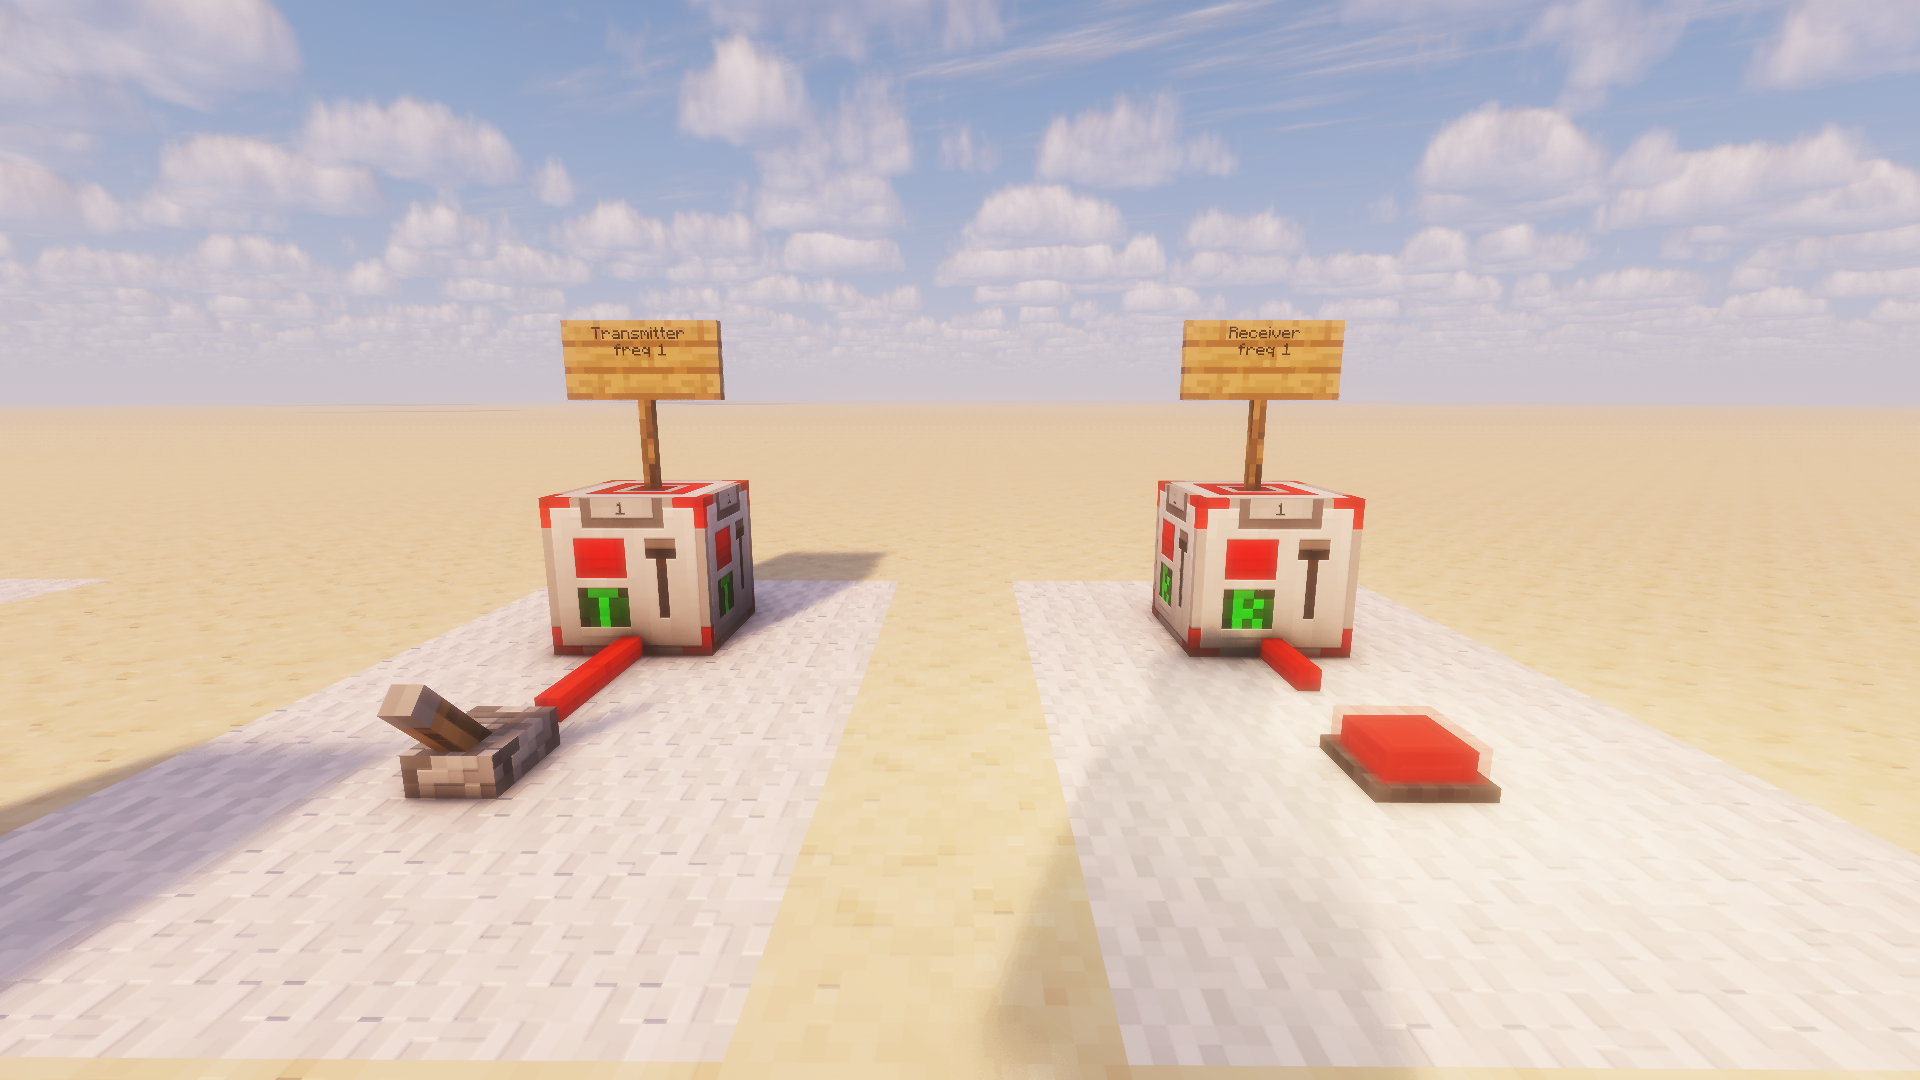
\includegraphics[width=0.7\linewidth]{images/wireless-redstone.png}
  	 \caption{Transmissor e Receptor}
   	\label{fig:wireless-redstone}
	%{\footnotesize Fonte: \url{https://autoctrls.com/datasheet-transistor/}}
\end{figure}